
\section{Určenie náklonu zbrane}
Pre určenie náklonu zbrane v~troch osách boli navrhnuté dve architektúry konvolučných neurónových sietí.
Každá z~týchto sietí bola natrénovaná tri-krát kvôli trom osiam rotácie.
Nastavenia sietí boli opísané v~návrhu.

Pre trénovanie v~osi pitch bolo použitých 1036 obrázkov, na validáciu 222 a taktiež 222 pre testovanie presnosti siete.
V~osi roll bolo na trénovanie použitých 3315 obrázkov, na validáciu 667 a 668 pre testovanie.
Nakoniec pre os yaw bolo použitých 3208 obrázkov na trénovanie a po 688 na validáciu a testovanie.
Všetky tieto obrázky prešli augmentáciou dát, ako je opísané v~\ref{subsec:augmentacia}.

\subsubsection{Pitch}
Siete boli trénovane v~50 epochách.
Priebeh trénovania obidvoch sietí pre os Pitch je vidieť na obrázku \ref{pic:pitchaxis}.
Kde pre presnosť týchto sietí je použitá metrika opísaná v~\ref{subsec:presnostmodelov}.
Hodnoty $angle\_error$ zobrazujú celkovú presnosť siete vzhľadom na priemernú odchýlku uhla pre trénovacie dáta,
    $val\_angle\_error$ určuje túto odchýlku pre validačné dáta.

\begin{figure}[H]
    \centering
    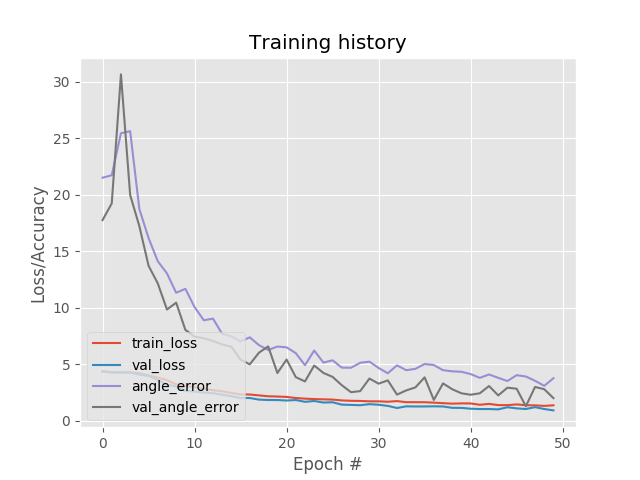
\includegraphics[width=0.49\textwidth]{alexnet-pitch5-training_history}
	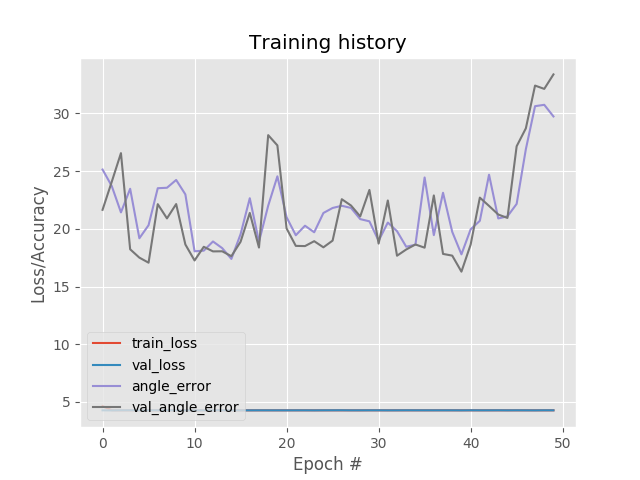
\includegraphics[width=0.49\textwidth]{vgglike-pitch5-training_history}
	\caption{Priebeh trénovania sietí AlexNetLike(vľavo) a VGGLike(vpravo).}
	\label{pic:pitchaxis}
\end{figure}

Výsledná presnosť sietí je uvedená v~tabuľkách \ref{tab:alexnetpitchresults} a \ref{tab:vgglikepitchresults} pre dve prahové hodnoty 5 a 10.

\begin{table}[H]
    \centering
    \begin{tabular}{|c|c|c|c|}
        \hline
        Prahová hodnota & V~prahovej hodnote       & Mimo prahovej hodnoty    & Úspešnosť    \\ \hline
        5               & {\color[HTML]{009901} 189} & {\color[HTML]{9A0000} 33} & \textbf{85.14\%} \\ \hline
        10              & {\color[HTML]{009901} 205} & {\color[HTML]{9A0000} 17} & \textbf{92.34\%} \\ \hline
    \end{tabular}
    \caption{Výsledky natrénovanej siete AlexNetLike pre os Pitch.}
    \label{tab:alexnetpitchresults}
\end{table}
\begin{table}[H]
    \centering
    \begin{tabular}{|c|c|c|c|}
        \hline
        Prahová hodnota & V~prahovej hodnote       & Mimo prahovej hodnoty    & Úspešnosť    \\ \hline
        5               & {\color[HTML]{009901} 9} & {\color[HTML]{9A0000} 213} & \textbf{4.05\%} \\ \hline
        10              & {\color[HTML]{009901} 17} & {\color[HTML]{9A0000} 205} & \textbf{7.66\%} \\ \hline
    \end{tabular}
    \caption{Výsledky natrénovanej siete VGGLike pre os Pitch.}
    \label{tab:vgglikepitchresults}
\end{table}


\subsubsection{Roll}
V~prípade AlexNetLike architektúry prebiehalo trénovanie rovnako ako v~prípade osi Pitch,
    avšak pri sietí VGGLike bolo potrebné znížiť počet interácií trénovania kvôli dlhej dobe
    spracovania jednej interácie, kedže trénovanie prebiehalo na väčšom počte dát oproti trénovaniu v~ose Pitch.
Aj z~priebehu trénovanie zobrazeného na obrázku \ref{pic:rollaxis} je možné vidieť že sieť veľmi nenapreduje k~lepším výsledkom.

\begin{figure}[H]
    \centering
    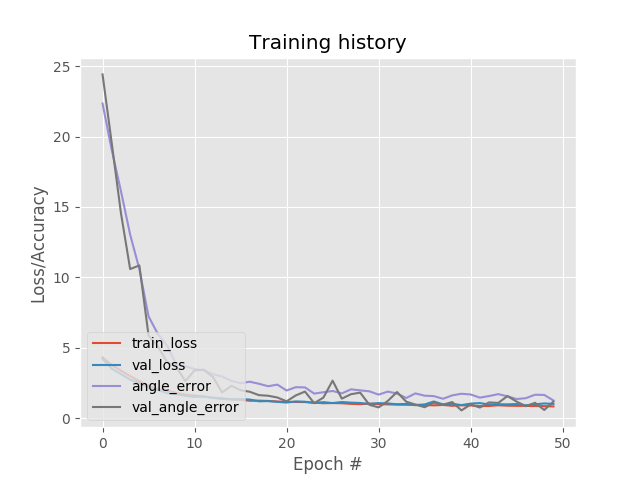
\includegraphics[width=0.49\textwidth]{alexnet-roll5-training_history}
	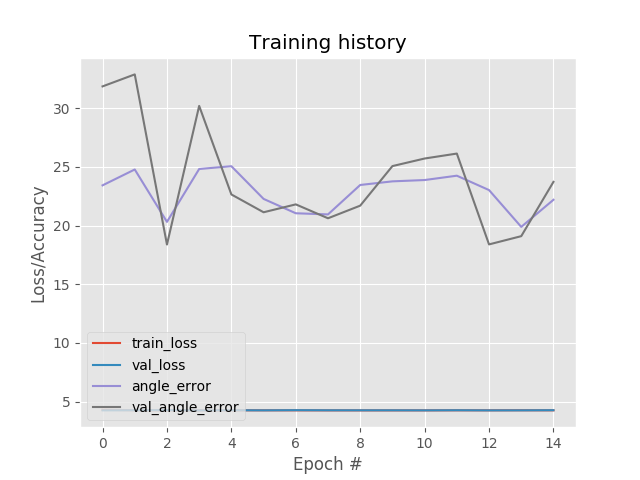
\includegraphics[width=0.49\textwidth]{vgglike-roll5-training_history}
	\caption{Priebeh trénovania sietí AlexNetLike(vľavo) a VGGLike(vpravo).}
	\label{pic:rollaxis}
\end{figure}

\begin{table}[H]
    \centering
    \begin{tabular}{|c|c|c|c|}
        \hline
        Prahová hodnota & V~prahovej hodnote       & Mimo prahovej hodnoty    & Úspešnosť    \\ \hline
        5               & {\color[HTML]{009901} 608} & {\color[HTML]{9A0000} 60} & \textbf{91.02\%} \\ \hline
        10              & {\color[HTML]{009901} 638} & {\color[HTML]{9A0000} 30} & \textbf{95.51\%} \\ \hline
    \end{tabular}
    \caption{Výsledky natrénovanej siete AlexNetLike pre os Roll.}
    \label{tab:alexnetrollresults}
\end{table}
\begin{table}[H]
    \centering
    \begin{tabular}{|c|c|c|c|}
        \hline
        Prahová hodnota & V~prahovej hodnote       & Mimo prahovej hodnoty    & Úspešnosť    \\ \hline
        5               & {\color[HTML]{009901} 25} & {\color[HTML]{9A0000} 643} & \textbf{3.74\%} \\ \hline
        10              & {\color[HTML]{009901} 36} & {\color[HTML]{9A0000} 632} & \textbf{5.39\%} \\ \hline
    \end{tabular}
    \caption{Výsledky natrénovanej siete VGGLike pre os Roll.}
    \label{tab:vgglikerollresults}
\end{table}


\subsubsection{Yaw}
Trénovanie pre os Yaw prebiehalo rovnako ako v~prípade osi Roll, počet epóch pre sieť VGGLike
    bol rovnako skrátený na 15 kvôli časovej náročnosti trénovania.

\begin{figure}[H]
    \centering
    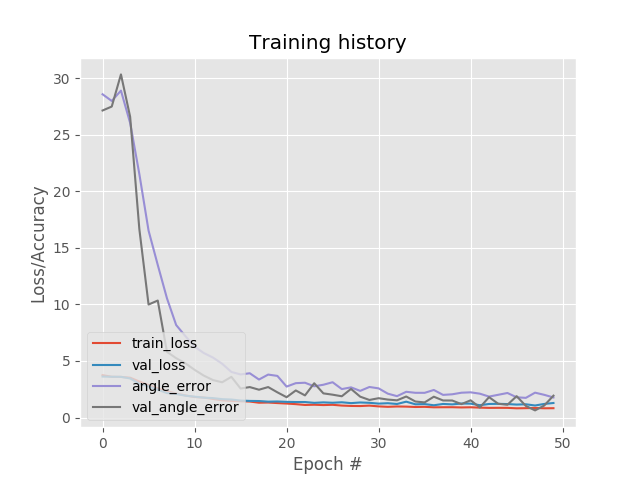
\includegraphics[width=0.49\textwidth]{alexnet-yaw5-training_history}
	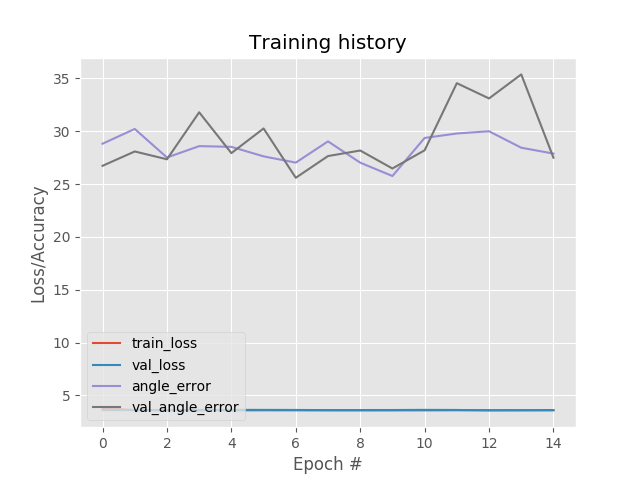
\includegraphics[width=0.49\textwidth]{vgglike-yaw5-training_history}
	\caption{Priebeh trénovania sietí AlexNetLike(vľavo) a VGGLike(vpravo).}
	\label{pic:yawaxis}
\end{figure}

\begin{table}[H]
    \centering
    \begin{tabular}{|c|c|c|c|}
        \hline
        Prahová hodnota & V~prahovej hodnote       & Mimo prahovej hodnoty    & Úspešnosť    \\ \hline
        5               & {\color[HTML]{009901} 342} & {\color[HTML]{9A0000} 346} & \textbf{49.71\%} \\ \hline
        10              & {\color[HTML]{009901} 376} & {\color[HTML]{9A0000} 312} & \textbf{54.65\%} \\ \hline
    \end{tabular}
    \caption{Výsledky natrénovanej siete AlexNetLike pre os Yaw.}
    \label{tab:alexnetyawresults}
\end{table}
\begin{table}[H]
    \centering
    \begin{tabular}{|c|c|c|c|}
        \hline
        Prahová hodnota & V~prahovej hodnote       & Mimo prahovej hodnoty    & Úspešnosť    \\ \hline
        5               & {\color[HTML]{009901} 26} & {\color[HTML]{9A0000} 662} & \textbf{3.78\%} \\ \hline
        10              & {\color[HTML]{009901} 41} & {\color[HTML]{9A0000} 647} & \textbf{5.96\%} \\ \hline
    \end{tabular}
    \caption{Výsledky natrénovanej siete VGGLike pre os Yaw.}
    \label{tab:vgglikeyawresults}
\end{table}
